In this section, 
I firstly introduce the adaptive data analysis, and the
%  cruciality 
significance for reasoning about the \emph{adaptivity} quantity property 
for adaptive data analysis program in Section~\ref{sec:adapt-background}.
% analyzing 
% Motivated by the significance of \emph{adaptivity},
% i
Then, in order to analyze this \emph{adaptivity} property for the adaptive data analysis,
there are three challenges
% problems encountered.
introduced in Section~\ref{sec:adapt-challenge}.
% I introduce these three problems
% and the full-spectrum analysis methodologies developed according to these problems 
Targeting to the three challenges, I give a short overview of the new proposed automatic analysis framework with respect to
the limitations of previous works.
%  Data analyses are usually designed to identify some property of the population from which the data are drawn, 
%  generalizing beyond the specific data sample. For this reason, data analyses are often designed in a way that guarantees that they produce a low generalization error.
%   That is, they are designed so that the result of a data analysis run on sample 
%   data does not differ too much from the result one would achieve by running the analysis over the entire population. 
The last part in Section~\ref{sec:adapt-outline} is an outline of this chapter with the contributions of this work.

 \subsection{Adaptive Data Analysis}
 \label{sec:adapt-background}The adaptive data analysis designed for identifying  properties for unknown populations / distributions 
 through data samples is widely 
 used in research and industrial areas.
 % , including machine learning areas, etc.. 
 When generalizing the analysis result from data samples to the unknown populations, 
 the generalization error is the key issue on which researchers are focusing to reduce.
 % Since An 
 Specifically in the adaptive data analysis,
 % the
 %  can be seen as 
 which is a process composed of 
 multiple queries interrogating some data
 %  in the analysis are , 
 % where 
 the choice of which query to run next may rely on the results of previous queries,
 the generalization error is propagated through the reliance between the choices of queries.
 In this sense, the \emph{adaptivity} rounds (i.e., how many queries are relied on others) in the analysis plays a key role in reducing the generalization error.
 Below I introduce in detail the adaptive data analysis procedure,
 and the significance of this \emph{adaptivity} quantity in effecting the generalization error.
 
 \paragraph{Adaptive Data Analysis Procedure}
 % \label{sec:intro-exelimitation}
 
 % Data analyses are usually designed to identify some property of the population 
 % from which the data are drawn, generalizing beyond the specific data sample. 
 % For this reason, data analyses are often designed in a way that guarantees that they produce a low generalization error.
 % That is, they are designed so that the result of a data analysis run on sample data does not differ too much from the result one would achieve by running the analysis over the entire population. 
 
 % An adaptive data analysis can be seen as a process composed of multiple queries interrogating some data, where the choice of which query to run next may rely on the results of previous queries. 
 % The generalization error of individual query/analysis can be controlled by using an array of well-established statistical techniques.
 % However, when queries are arbitrarily composed, the different errors can propagate through the chain of different queries and bring high generalization errors. 
 % To address this issue, data analysts are designing several techniques that not only guarantee bounds on the generalization errors of single queries, but also guarantee bounds on the generalization error of the composed analyses. 
 % The choice of which of these techniques to use, 
 % often depends on the chain of queries that an adaptive data analysis can generate.
 % Specifically, the total number of queries and the depth of the chain of queries is of great significance 
 % to guarantee the generalization error, 
 % when the composed data analyses are adaptive. 
 % So in order to give a precise guarantee of generalization error
 % for the program,
 % I'm interested in analyzing the depth of the chain of queries in a program, i.e., the program's \emph{adaptivity} property.
 
 Consider a dataset $X$ consisting of $n$ independent samples from some unknown population $\dist$. How can I ensure that the conclusions are drawn from $X$ \emph{generalize} to the population $\dist$? Despite decades of research in statistics and machine learning on methods for ensuring generalization, there is an increased recognition that many scientific findings generalize poorly (e.g. 
 \cite{Ioannidis05,GelmanL13}
 ). While there are many reasons a conclusion might fail to generalize, one that is receiving increasing attention is \emph{adaptivity}, which occurs when the choice of method for analyzing the dataset depends on previous interactions with the same dataset~\cite{GelmanL13}.
 
  Adaptivity can arise from many common practices, such as exploratory data analysis, using the same data set for feature selection and regression, and the re-use of datasets across research projects. Unfortunately, adaptivity invalidates traditional methods for ensuring generalization and statistical validity, which assume that the method is selected independently of the data. The misinterpretation of adaptively selected results has even been blamed for a ``statistical crisis'' in empirical science~\cite{GelmanL13}.
 % ~\cite{GelmanL13}.
 
 A line of work initiated by \cite{DworkFHPRR15}, \cite{HardtU14} posed the question: 
 Can I design \emph{general-purpose} methods that ensure generalization in the presence of adaptivity, together with guarantees on their accuracy? 
 The idea that has emerged in these works is to use randomization to help ensure generalization. 
 Specifically, these works have proposed to mediate the access of an adaptive data analysis to the data utilizing queries from some pre-determined family (I will consider here a specific family of queries often called "statistical" or "linear" queries) that are sent to a 
 \emph{mechanism} which uses some randomized process to guarantee that the result of the query does not depend too much on the specific
 sampled dataset. 
 %
 \begin{figure}
  \centering
  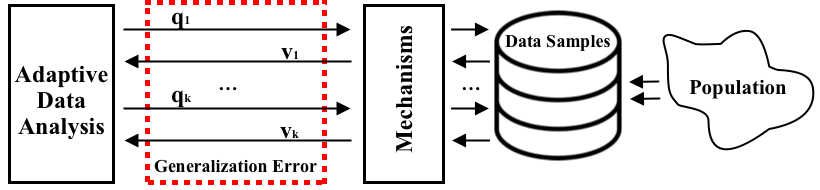
\includegraphics[width=0.7\columnwidth]{figures/data_analysis_model.png}
  \caption{Overview of our Adaptive Data Analysis model.}
  \label{fig:adaptivity-model-overview}
 \vspace{-0.5cm}
 \end{figure}
 This guarantees that the result of the queries generalizes well. 
 This approach is described in Figure~\ref{fig:adaptivity-model-overview}, where
 I have a population that I am interested in studying, and a dataset containing individual samples from this population. The adaptive data analysis I am interested in running has access to the dataset through queries of some pre-determined family (e.g., statistical or linear queries) mediated by a mechanism. 
 This mechanism uses randomization to reduce the generalization error of the queries issued to the data.
 This line of work has identified many new algorithmic techniques for ensuring generalization in adaptive data analysis, leading to algorithms with greater statistical power than all previous approaches. 
 Common methods proposed by these works include the addition of noise to the result of a query, data splitting, etc. 
 Moreover, these works have also identified problematic strategies for adaptive analysis, showing limitations on the statistical power one can hope to achieve. 
 Subsequent works have then further extended the methods and techniques in this approach and further extended the theoretical underpinning of this approach, 
 e.g.~\cite{dwork2015reusable,dwork2015generalization,BassilyNSSSU16,UllmanSNSS18,FeldmanS17,jung2019new,SteinkeZ20,RogersRSSTW20}.
 %
 
 A key development in this line of work is that the best method for ensuring generalization in an adaptive data analysis depends to a large extent on the number of \emph{rounds of adaptivity}, the depth of the chain of queries. 
 As an informal example, the program $x \leftarrow \query_1(D);y \leftarrow \query_2(D,x);z \leftarrow \query_3(D,y)$ has three rounds of adaptivity, since $\query_2$ depends on $D$ not only directly because it is one of its input but also via the result of $\query_1$, 
 which is also run on $D$, and similarly, $\query_3$ depends on $D$ directly but also via the result of $\query_2$, which in turn depends on the result of $\query_1$. 
 The works I discussed above showed that not only does the analysis of the generalization error depend on the number of rounds, 
 but knowing the number of rounds allows one to choose methods that lead to the smallest possible generalization error. 
 
 % \mg{Check the following - also the plots need to be on the same scale!}
 For example, these works showed that when an adaptive data analysis uses a large number of rounds 
 of adaptivity then a low generalization error can be achieved by the mechanism that 
 adds Gaussian noise scaled to the number of rounds to each query result.
 When instead an adaptive data analysis uses a small number of rounds of adaptivity then a low generalization error can be achieved by using more specialized methods, such as the data splitting mechanism or the reusable holdout technique from~\cite{DworkFHPRR15}.
 To better understand this idea, I show in Figure~\ref{fig:generalization_errors} two experiments showcasing these situations. 
 More precisely, in Figure~\ref{fig:generalization_errors}(a) shows the results of a real-world analysis
 with two rounds of adaptivity. 
 This analysis can be seen as a classifier that first runs 500 non-adaptive queries on the first 500 attributes of the data, looking for correlations between the attributes and a label, and then runs one last query which depends on all these correlations. 
 Without any mechanism, the generalization error is pretty large, and the lower generalization error is achieved when the data-splitting method is used. 
 In Figure~\ref{fig:generalization_errors}(b) shows the results of a specific analysis
 with four hundred rounds of adaptivity. 
 This analysis can be seen as a classifier that at each step runs an adaptive query based on the result of the previous ones. 
 Again, without any mechanism, the generalization error is pretty large, and the lower generalization error is achieved when the Gaussian noise is used. 
 {\small
 \begin{figure}
 \centering
 \begin{subfigure}{.48\textwidth}
 \begin{centering}
 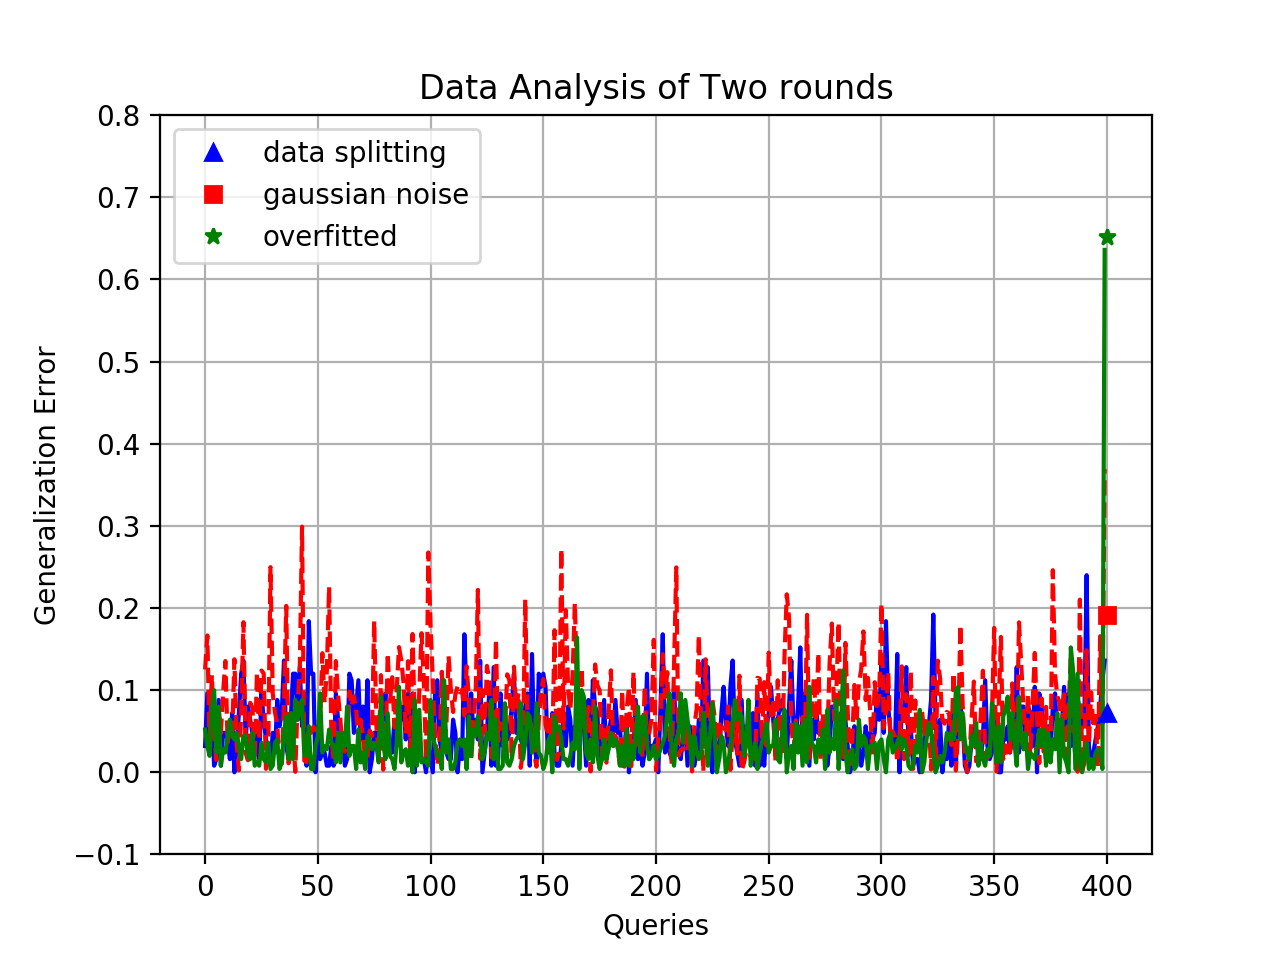
\includegraphics[width=0.9\textwidth]{figures/tworound.png}
 \caption{}
 \end{centering}
 \end{subfigure}
 %}
 \quad
 \begin{subfigure}{.48\textwidth}
 \begin{centering}
 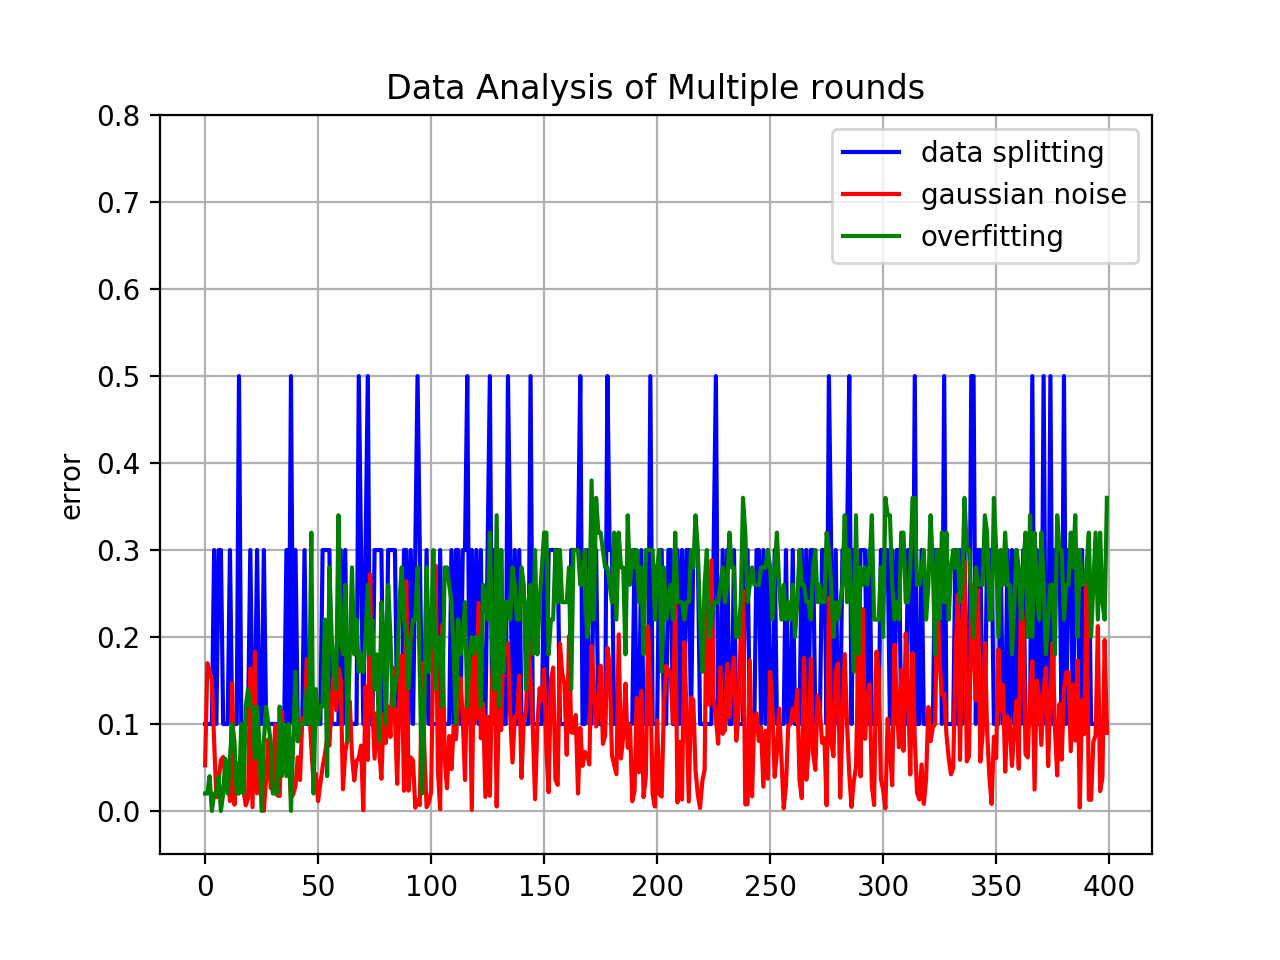
\includegraphics[width=0.9\textwidth]{figures/multipleround.png}
 \caption{}
 \end{centering}
 \end{subfigure}
 \vspace{-0.4cm}
  \caption{
  The generalization errors of two adaptive data analysis examples, under different choices of mechanisms.
  (a) Data analysis with adaptivity 2, 
  (b) Data analysis with adaptivity 400. 
 }
 \label{fig:generalization_errors}
 \vspace{-0.5cm}
 \end{figure}
 }
 %gap
 This scenario motivates us to explore the design of program analysis techniques that can be used to estimate the number of \emph{rounds of adaptivity} that a program implementing a data analysis can perform. These techniques could be used to help a data analyst in the choice of the mechanism to use,
 and they
 could ultimately be integrated into a tool for adaptive data analysis such as the \emph{Guess and Check} framework by~\cite{RogersRSSTW20}. 
 %
\subsection{Challenges}
\label{sec:adapt-challenge}
Given the significance of this \emph{adaptivity} quantity in data analysis area,
I'm motivated to analysis this property.
In order to analyze this property, there is mainly three challenges introduced below.
%  in Section~\ref{sec:adapt-intro-challenge}.
Then targeting to the three challenges, I give a short overview of the new proposed adaptivity analysis framework
with respect to the limitations of previous works.

\begin{enumerate}
 \item
 \textbf{Adaptive Data Analysis Formalization}

The first challenge is \emph{how to define formally} a model for adaptive data analysis which is general enough to support the methods I discussed above and would permit to formulate the notion of adaptivity these methods use. 
I take the approach of designing a programming framework for submitting queries to some \emph{mechanism} giving access 
to the data mediated by one of the techniques which are mentioned before, 
including the mechanism of adding Gaussian noise, 
the mechanism that randomly selects a subset of the data, 
and the mechanism that uses the reusable holdout technique, etc. 
In this approach, a program models an \emph{analyst} asking a sequence of queries to the mechanism. 
The mechanism runs the queries on the data applying one of the methods discussed above and returns the result to the program. The program can then use this result to decide which query to run next. 
% Overall, I am interested in controlling the generalization of the results of the queries which are returned by the mechanism, by means of adaptivity. 

% \textbf{Methodology}
% There are previous works from \todo{Thesis} developing language formalizing the adaptive data analysis.
% However, their formalization is limited in the expressiveness largely.
Motivated by this, I present a new while-like language 
named {\tt Query While} language with extensions on query requests in Section~\ref{sec:adapt-language}.

\item 
\textbf{Adaptivity Formalization}

The second challenge is \emph{how to define the adaptivity of a given program}.
Intuitively, a query $Q$ may depend on another query $P$, if there are two values that $P$ can return which affect in different ways the execution of $Q$. 
For example, as shown in \cite{dwork2015reusable}, and as I did in our example in Figure~\ref{fig:generalization_errors}(a), one can design a machine learning algorithm for constructing a classifier that first computes each feature's correlations with the label via a sequence of queries, and then constructs the classifier based on the correlation values. 
If one feature's correlation changes, the classifier depending on features is also affected. 
This notion of dependency builds on the execution trace as a \emph{causal history}. 
In particular, I am interested in the history or provenance of a query up until this is executed, 
% I am not then concerned about how the result is used --- except for 
simultaneously in tracking whether the result of the query may further cause some other query. 
This is because I'm focusing on the generalization error which could be propagated by queries.
% and not their post-processing. % 

To formalize this intuitive \emph{adaptivity} as a quantitative program property, 
I present an adaptivity definition in Section~\ref{sec:adapt-exe} based on the language and semantics.
% \textbf{Methodology}
% % I first consider all the possible evaluations of a program --- I do this by 
% % I use a trace semantics recording the execution history of programs on some given input --- and I create a dependency graph, where the dependency between different variables (query is also assigned to a variable) is explicit and track which variable is associated with a query request. 
% % I then enrich this graph with weights describing the maximal number of times each variable is evaluated in a program evaluation starting with an initial state. The adaptivity is then defined as the length of the walk visiting most query-related variables on this graph. 
% % Through two aspects: the execution-based analysis and static-based program analysis.
% % In the execution-based analysis, I will formalize the intuitive notion of \emph{adaptivity} as a quantitative 
% % property of programs. This analysis is developed 
%  This execution-based analysis is designed in three steps through different methodologies as follows,
%  \begin{enumerate}
%  \item The first step is to analyze the \emph{dependency relation} between every query, 
%  through the methodology of semantic data dependency analysis.
%  %
%  Specifically through a trace semantics recording the execution history of programs on given input,
%  % --- and I create a dependency graph, 
%  the dependency between different variables (query is also assigned to a variable) is explicitly tracked and 
%  analyzed.
% %   and 
% %   which variable is associated with a query request. 
% % I then enrich this graph with weights describing the maximal number of times each variable is evaluated in a program evaluation starting with an initial state. The adaptivity is then defined as the length of the walk visiting most query-related variables on this graph. 
% % In the execution-based analysis, I will formalize the intuitive notion of \emph{adaptivity} as a quantitative 
% % property of programs. This analysis is developed 
% % \\
%  \item The second step is to analyze the \emph{dependency quantity} 
% %  analysis, 
% based on the \emph{dependency relation} above.
% This analysis is developed through the methodology of execution-based reachability bound analysis.
% % \\
%  \item The last step is the intuitive \emph{adaptivity} quantity analysis, 
%  according to the two analysis results above, specifically \emph{dependency relation} and \emph{dependency quantity}.
%  This step 
% %  is developed through 
% gives the formal \emph{adaptivity} definition as the analysis result. \\
%  Specifically, this analysis is developed through creating a dependency graph firstly. 
%  In this graph, the dependency between different variables (query is also assigned to a variable) 
%  is explicit and track which variable is associated with a query request. 
%  This dependency comes from the \emph{dependency relation} from the first step analysis.
%  \\
% Then, I enrich this graph with 
% weights describing the maximal number of times each variable is evaluated in a program evaluation starting with an initial state. 
% This weight comes from the \emph{dependency quantity} from the second step analysis results.
% \\
%  The adaptivity is then defined as the length of the walk visiting most query-related variables on this graph. 
%  \end{enumerate}
\item 
\textbf{Adaptivity Estimation}

The third challenge is \emph{how to estimate the adaptivity of a given program}. 
The adaptive data analysis model I consider and our definition of adaptivity suggest that for this task 
I can use a program analysis that is based on some form of dependency analysis.
 This analysis needs to take into consideration:
1) the fact that, in general, a query $Q$ is not a monolithic block but rather it may depend, through the use of variables and values, on other parts of the program. 
Hence, it needs to consider some form of data flow analysis. 
2) the fact that, in general, the decision on whether to run a query or not may depend on some other value. Hence, 
 it needs to consider some form of control flow analysis.
3) the fact that. in general, I am not only interested in whether there is a dependency or not, but in the length of the chain of dependencies. 
Hence, it needs to consider some quantitative information about the program dependencies. % {A quick example is that: I store the result of query $Q_1$ in variable $x$ and use variable $y$ to record the result of query $Q_2$. I want to construct the third query $Q_3$ which relies on the value stored in $x$, let us say, $Q_3$ will ask for the sum of the first column of a table if $x$ is positive and the sum of the second column otherwise. In this situation, I need data flow analysis. On the other hand, if I need the value of $y$ to help us decide whether I should ask $Q_3$, for example, I ask the third query if $y$ is odd, and do not ask if $y$ is even. Naturally, to be able to handle this case, control flow analysis comes into play. Formally speaking, }

To address these considerations and be able to estimate a sound upper bound on the adaptivity of a program, 
I propose a static program analysis in Section~\ref{sec:adapt-static}, named {\THESYSTEM}.
%%%%% To reason about%
\end{enumerate}

In summary, this new program analysis framework is
%  developed
%  full-spectrum analysis of this property is 
% In this proposal, I will first focus on analyzing 
% this adaptivity property for the program based on solving 
developed w.r.t. the three challenges accordingly,
through the three parts:
the language formalization,
the formal adaptivity definition and the static program analysis algorithm estimating adaptivity.


\subsection{Outline}
\label{sec:adapt-outline}
The rest parts of this section is organized as follows. 
\begin{enumerate}
   \item The previous works on adaptive data analysis are introduced in Section~\ref{sec:prework}.
   \item The proposed new program analysis framework for the adaptivity of Adaptive Data Analysis is presented 
   in Section~\ref{sec:adapt-analysis}.
   This new program analysis framework has three major components:
   \begin{enumerate}
      \item A while-like language extended with query request feature, named {\tt Query While} Language  in Section~\ref{sec:adapt-language}, 
      used to implement the adaptive data analysis;
      \item A formal adaptivity definition in Section~\ref{sec:adapt-exe};
      \item A static program analysis algorithm, named {\THESYSTEM} through static adaptivity analysis in Section~\ref{sec:adapt-static}.
   \end{enumerate}
\end{enumerate}